\chapter{Checkerboard}
\label{c-checkers}
%\Chapter{checkers}{28jan2018}{Checkerboard}
%\label{c-checkers}  % formatted for ChaosBook.org
%\listofsections{0}
% siminos/spatiotemp/chapter/checkers.tex
% $Author: predrag $ $Date: 2019-05-09 18:30:52 -0400 (Thu, 09 May 2019) $


\section{Checkerboard model}
\label{sect:checkers}

\begin{description}

    \item[2019-03-08 Zeb]
Rodrigues \etal\rf{RFSP17} looks very interesting.

I'm interested in whether the nonlinearities of these
flexible structures can lead to interesting chaotic behavior. The thing
foremost on my mind is the structure (not dynamics) of a 1D chain of
repeating mechanical elements. A rigid-body mechanism would lead to a
nonlinear transfer function between the configuration of one element and
its neighbors. That seems like it could lead to something like the
logistic equation, and perhaps different structures depending on the
shape of the unit cell and the ``initial" (\ie, boundary) conditions.

I couldn't get that to work out, but Michael, see
\reffig{fig:checkersChaos}\,(a), found something that suggests it could
work. Specifically, he found a structure that is repeated every three
unit cells.

Two-dimensional structures like the origami are also quite interesting,
of course, but the 1D chain seems easier to us as a starting point.

    \item[2019-03-08 Adrian]
James McInerney work is focused on origami.


%%%%%%%%%%%%%%%%%%%%%%%%%%%%%%%%%%%%%%%%%%%%%%%%%%%%%%
\begin{figure}[h]
    \begin{center}
%\begin{minipage}[height=.20\textheight]{.18\textwidth}
%\centering
%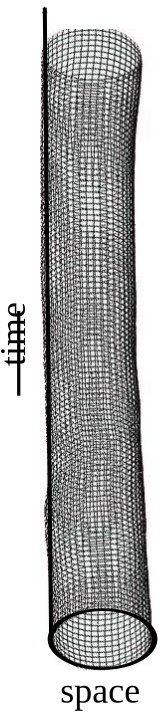
\includegraphics[width=.75\textwidth]{cylinderTime1}
%    \vfill
%\small{\texttt{(a)}}
%\end{minipage}
%~~~~
\begin{minipage}[height=.20\textheight]{.75\textwidth}
\centering
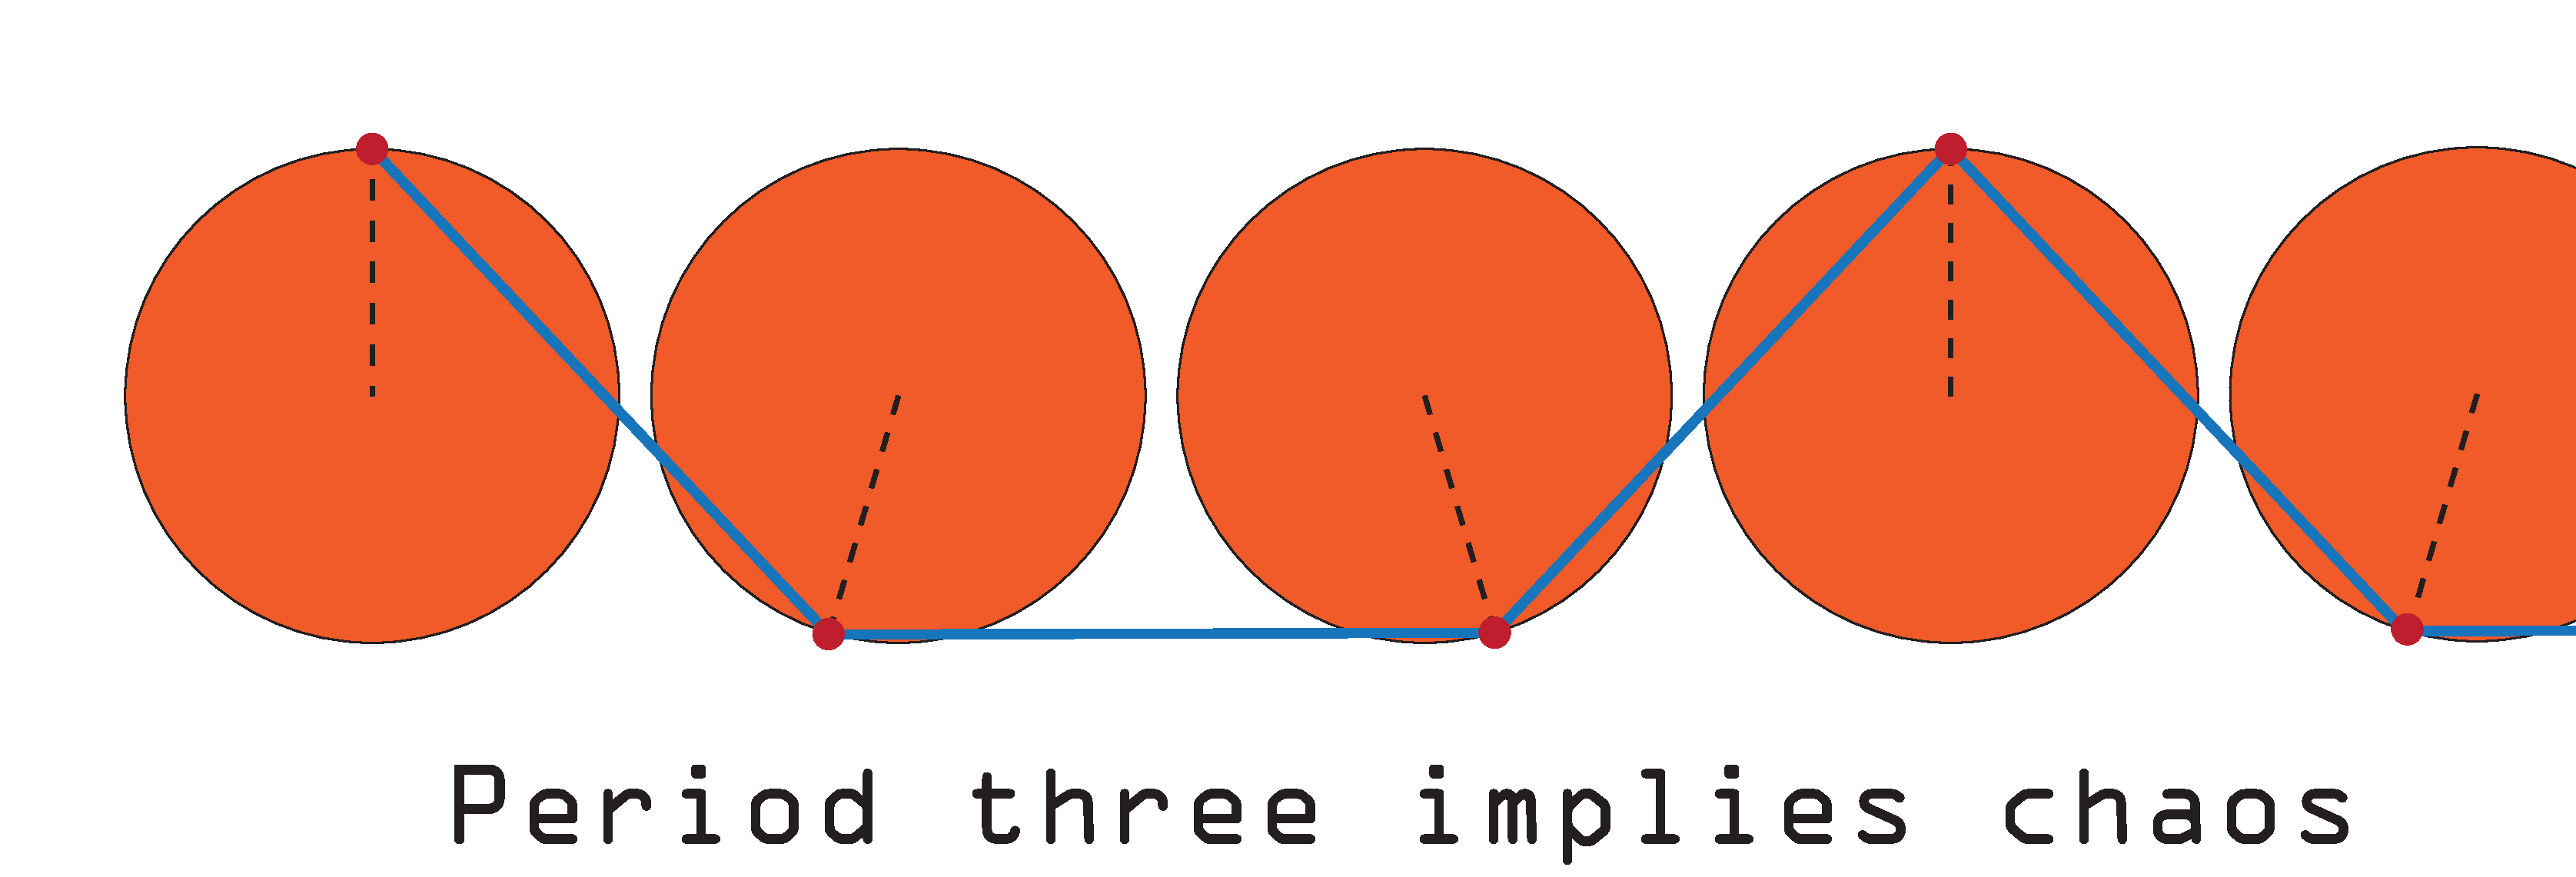
\includegraphics[width=.86\textwidth]{checkersChaosOrig}
\\
\small{\texttt{(a)}}
\\
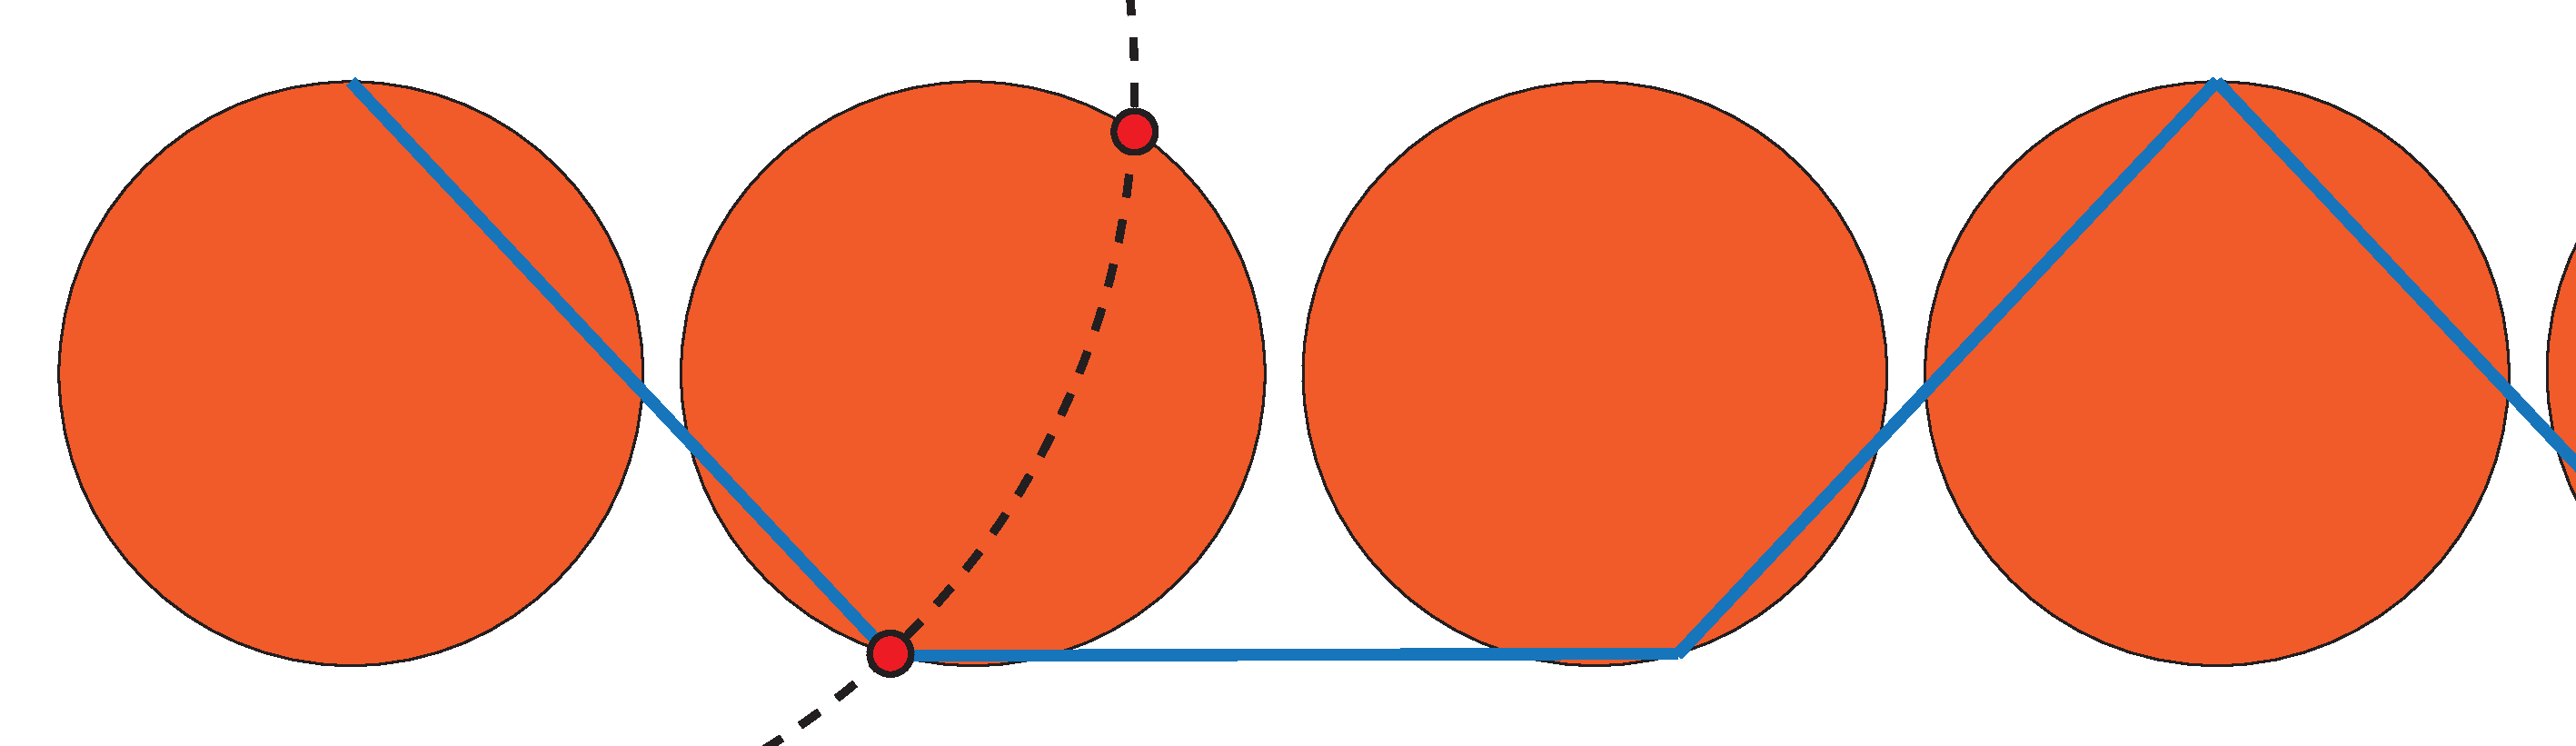
\includegraphics[width=.80\textwidth]{checkersChaosDegen}
\\
\small{\texttt{(b)}}
\end{minipage}
    \end{center}
\caption{\label{fig:checkersChaos}
(a)
    The wheels on a steam engine, with the rod lengths varied around to
    produce a mismatch.
(b)
    Forward-iteration almost always has two solutions, as there are two
    points at which the two circles intersect.
}
\end{figure}
%%%%%%%%%%%%%%%%%%%%%%%%%%%%%%%%%%%%%%%%%%%%%%%%%%%%%%

    \item[2019-03-08 Michael D. Czajkowski]
<michael.czajkowski@physics.gatech.edu>\\
I have located a configuration of a chain of 1-d rotors which repeats in
three cycles, see \reffig{fig:checkersChaos}\,(a).

It is not unlike the wheels on a classical
steam engine, but with the rod lengths varied around to produce a
mismatch.  We are thinking, of course, of the sequence of rotors going
from left to right (or vice versa) as like time going forward in the
iterative cycles of the logistic map.
Despite the simplicity it seems promising in identifying a
deterministic geometric system, which will never repeat, by varying the
intrinsic parameters (like the rotor radius, connector length, etc).

There is one caveat to this, which is that we are thinking of the (for
instance) orientation of the leftmost rotor as the input which (together
with the intrinsic length of our blue rod, the radius of the orange
circles and the spacing between them) determines the next orientation of
the following rod to the right of it. However, this almost always has two
solutions, as there are two points at which the two circles intersect,
see \reffig{fig:checkersChaos}\,(b). So we are not entirely sure yet how
to think of determinism in this system. Perhaps that is a bad
thing, or perhaps it will be an interesting source of additional
richness.

There is a separate perspective on this same mechanical system where
there may be an analogue of chaos in a correspondence with topological
mechanical polarization, but this is less developed and I will wait to
share until I have gathered my thoughts a bit more.


\end{description}

\subsection{Checkerboard literature}
\label{sect:checkersLit}


\hfill   {\color{red} For the latest entry, go to the bottom of this section}

\bigskip


\begin{description}

    \item[2019-03-08 Predrag]
Rodrigues, Fonseca, Savi and Paiva\rf{RFSP17}
{\em Nonlinear dynamics of an adaptive origami-stent system}

\end{description}

%%%%%%%%%%%%%%%%%%%%%%%%%%%%%%%%%%%%%%%%%%%%%%%%
\printbibliography[heading=subbibintoc,title={References}]

\ChapterEnd % formatted for ChaosBook.org
